\documentclass[11pt]{article}
\usepackage[utf8]{inputenc}
\usepackage[T1]{fontenc}
\usepackage[spanish]{babel}
\usepackage{amsmath}
\usepackage{booktabs}
\usepackage{graphicx}
\usepackage{float}
\usepackage{geometry}
\geometry{margin=2.5cm}
\setlength{\parskip}{0.65em}
\setlength{\parindent}{0pt}
\title{Informe de resultados Desempleo macro - abandono V1}
\author{FinPUC}
\date{}
\begin{document}
\maketitle
\section{Análisis de resultados fuera de muestra}
Esta iteracion calibra y valida la view \textit{Desempleo macro} bajo la arquitectura robustecida de tres horizontes. La configuracion congelada resultante corresponde a familia unemployment, lookback 252 dias, ponderacion equal, q\_scale=1.5, confianza=50\% y $\tau$=0.200. La capa P4 usa la Version 1 de abandono: $p_{retiro,t}=0$ si $loss_t\leq\hat{x}_1$ y $p_{retiro,t}=[1+\exp(-(loss_t-\hat{x}_1))]^{-1}$ si $loss_t>\hat{x}_1$.
\begin{table}[H]
\centering
\resizebox{\textwidth}{!}{%
\begin{tabular}{lrrrrrrr}
\toprule
Escenario & Perfil & Sharpe BL & Sharpe MK & Mejora Sharpe & DD BL & DD MK & \% recomendado \\
\midrule
sin\_pandemia & Muy conservador & 1.738 & 1.736 & 0.2\% & -10.2\% & -10.3\% & 100.0\% \\
sin\_pandemia & Conservador & 1.718 & 1.728 & -0.6\% & -10.1\% & -11.0\% & 0.0\% \\
sin\_pandemia & Neutro & 1.664 & 1.747 & -4.8\% & -10.2\% & -13.0\% & 0.0\% \\
sin\_pandemia & Arriesgado & 1.562 & 1.513 & 3.2\% & -12.1\% & -18.2\% & 100.0\% \\
sin\_pandemia & Muy arriesgado & 1.154 & 1.198 & -3.7\% & -21.1\% & -26.5\% & 0.0\% \\
con\_pandemia & Muy conservador & 1.625 & 1.699 & -4.4\% & -9.1\% & -9.0\% & 0.0\% \\
con\_pandemia & Conservador & 1.638 & 1.749 & -6.5\% & -9.2\% & -9.0\% & 0.0\% \\
con\_pandemia & Neutro & 1.660 & 1.773 & -6.0\% & -9.4\% & -10.9\% & 25.0\% \\
con\_pandemia & Arriesgado & 1.644 & 1.391 & 19.9\% & -11.1\% & -18.7\% & 75.0\% \\
con\_pandemia & Muy arriesgado & 1.119 & 0.933 & 23.1\% & -22.8\% & -27.6\% & 100.0\% \\
\bottomrule
\end{tabular}
}
\caption{Comparacion fuera de muestra para Desempleo macro con abandono V1.}
\label{tab:desempleo_macro_v1:oos}
\end{table}

\section{Resultados de la dinámica de portafolio}
La dinamica del portafolio se evalua antes de la simulacion economica para separar el comportamiento financiero del modelo de la respuesta conductual del cliente. El turnover semestral, el numero efectivo de activos y la concentracion sectorial permiten medir si la view es implementable sin exigir cambios excesivos de composicion.
\begin{table}[H]
\centering
\resizebox{\textwidth}{!}{%
\begin{tabular}{lrrrrrr}
\toprule
Escenario & Perfil & Turnover & Turn. >20\% & N efectivo & HHI sector & Peso sector lider \\
\midrule
sin\_pandemia & Muy conservador & 7.0\% & 0.0\% & 221.21 & 0.147 & 27.5\% \\
sin\_pandemia & Conservador & 7.0\% & 0.0\% & 233.51 & 0.144 & 27.2\% \\
sin\_pandemia & Neutro & 6.9\% & 0.0\% & 271.13 & 0.137 & 26.2\% \\
sin\_pandemia & Arriesgado & 6.9\% & 0.0\% & 360.45 & 0.124 & 21.8\% \\
sin\_pandemia & Muy arriesgado & 9.2\% & 0.0\% & 163.27 & 0.178 & 32.1\% \\
con\_pandemia & Muy conservador & 6.3\% & 0.0\% & 112.55 & 0.169 & 25.7\% \\
con\_pandemia & Conservador & 6.2\% & 0.0\% & 118.08 & 0.166 & 25.0\% \\
con\_pandemia & Neutro & 6.4\% & 0.0\% & 136.34 & 0.158 & 23.5\% \\
con\_pandemia & Arriesgado & 7.0\% & 0.0\% & 205.71 & 0.135 & 20.1\% \\
con\_pandemia & Muy arriesgado & 9.9\% & 0.0\% & 120.96 & 0.214 & 37.9\% \\
\bottomrule
\end{tabular}
}
\caption{Dinamica de portafolio de Black-Litterman para Desempleo macro.}
\label{tab:desempleo_macro_v1:dinamica}
\end{table}

\section{Evaluación Económica Monte Carlo P4 en Horizonte Limpio}
La simulacion Monte Carlo P4 se ejecuta solo en el horizonte limpio, con 2000 trayectorias por cruce modelo-escenario-perfil y 260 semanas. La utilidad de empresa es ex-post y corresponde al 0,5\% mensual del saldo administrado activo. El abandono se calcula semanalmente y se reporta tambien en equivalente semestral.
\begin{table}[H]
\centering
\resizebox{\textwidth}{!}{%
\begin{tabular}{lrrrrrrrrr}
\toprule
Escenario & Perfil & Riqueza & Utilidad & P acepta reb. & P abandono semanal & P abandono sem. & Retiro 260w & Retencion & Clientes finales \\
\midrule
sin\_pandemia & Muy conservador & 1.434 & 124 & 55.7\% & 0.6\% & 14.3\% & 34.4\% & 38.7\% & 434 \\
sin\_pandemia & Conservador & 1.839 & 250 & 54.3\% & 0.1\% & 1.8\% & 7.8\% & 85.6\% & 931 \\
sin\_pandemia & Neutro & 1.880 & 266 & 51.6\% & 0.0\% & 0.0\% & 0.2\% & 99.6\% & 1033 \\
sin\_pandemia & Arriesgado & 1.810 & 248 & 47.9\% & 0.0\% & 0.0\% & 0.0\% & 100.0\% & 965 \\
sin\_pandemia & Muy arriesgado & 1.863 & 246 & 46.0\% & 0.0\% & 0.0\% & 0.1\% & 99.8\% & 925 \\
con\_pandemia & Muy conservador & 1.313 & 105 & 54.9\% & 0.7\% & 16.0\% & 35.5\% & 36.0\% & 399 \\
con\_pandemia & Conservador & 1.709 & 234 & 53.7\% & 0.1\% & 1.7\% & 8.1\% & 85.2\% & 927 \\
con\_pandemia & Neutro & 1.775 & 253 & 51.3\% & 0.0\% & 0.0\% & 0.3\% & 99.5\% & 1025 \\
con\_pandemia & Arriesgado & 1.774 & 240 & 47.9\% & 0.0\% & 0.0\% & 0.0\% & 100.0\% & 946 \\
con\_pandemia & Muy arriesgado & 1.956 & 257 & 46.2\% & 0.0\% & 0.0\% & 0.2\% & 99.7\% & 926 \\
\bottomrule
\end{tabular}
}
\caption{Resultados P4 para Desempleo macro con abandono V1.}
\label{tab:desempleo_macro_v1:p4}
\end{table}

\begin{figure}[H]
\centering
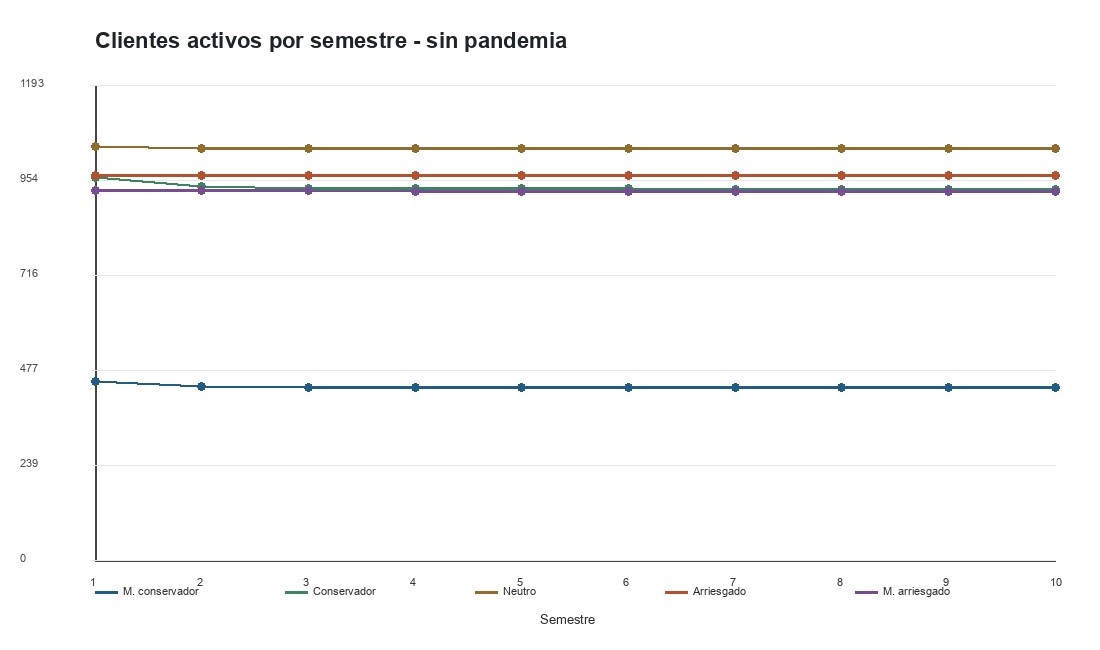
\includegraphics[width=0.86\textwidth]{figuras/serie_clientes_sin_pandemia.png}
\caption{Clientes activos por semestre sin pandemia para Desempleo macro con abandono V1.}
\label{fig:desempleo_macro_v1:clientes_sin}
\end{figure}
\begin{figure}[H]
\centering
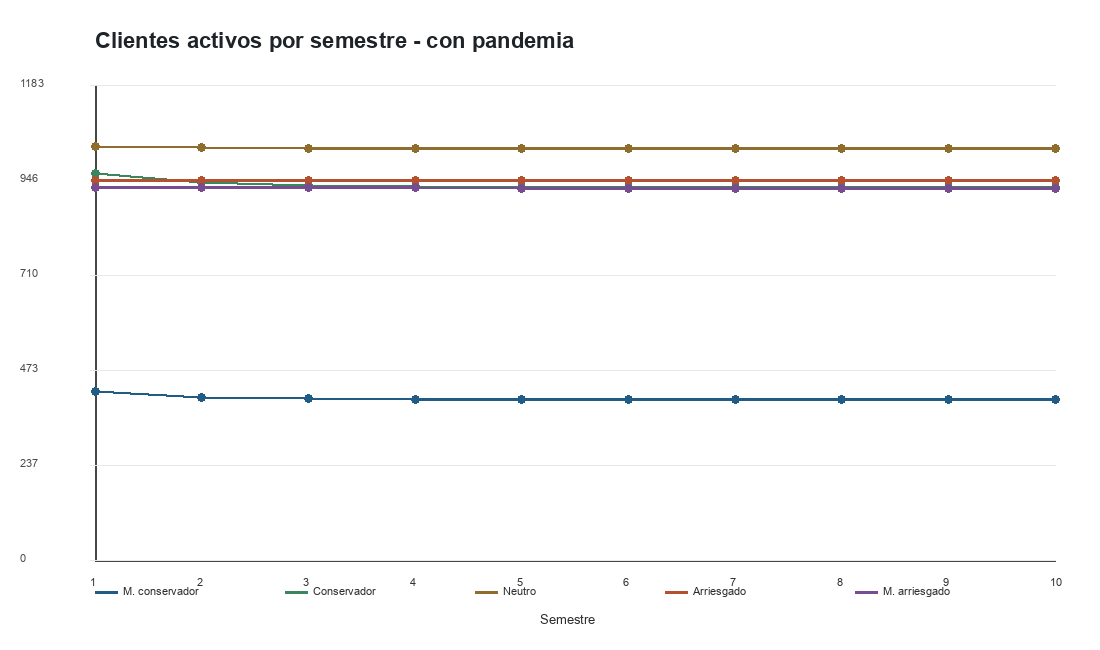
\includegraphics[width=0.86\textwidth]{figuras/serie_clientes_con_pandemia.png}
\caption{Clientes activos por semestre con pandemia para Desempleo macro con abandono V1.}
\label{fig:desempleo_macro_v1:clientes_con}
\end{figure}
\begin{figure}[H]
\centering
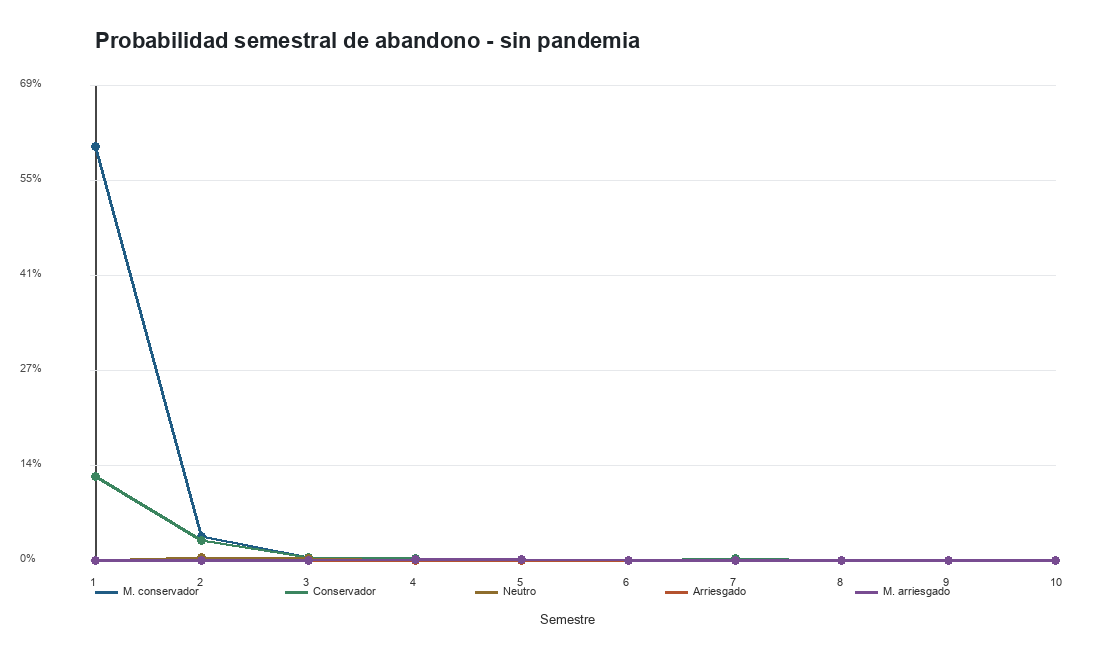
\includegraphics[width=0.86\textwidth]{figuras/serie_abandono_sin_pandemia.png}
\caption{Probabilidad semestral de abandono sin pandemia para Desempleo macro con abandono V1.}
\label{fig:desempleo_macro_v1:abandono_sin}
\end{figure}
\begin{figure}[H]
\centering
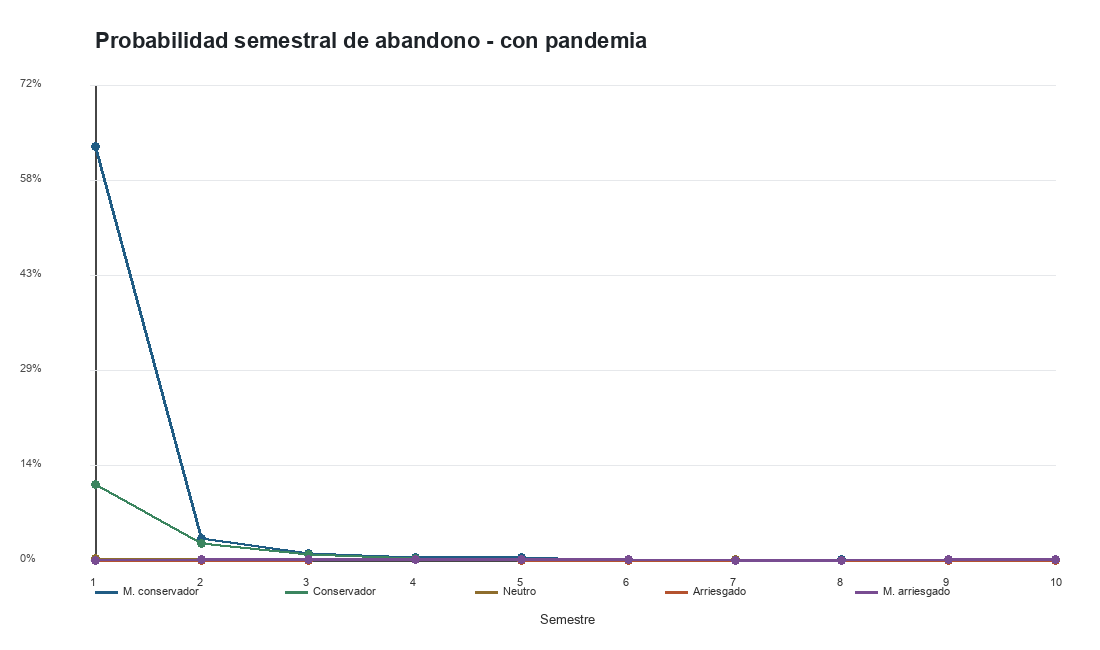
\includegraphics[width=0.86\textwidth]{figuras/serie_abandono_con_pandemia.png}
\caption{Probabilidad semestral de abandono con pandemia para Desempleo macro con abandono V1.}
\label{fig:desempleo_macro_v1:abandono_con}
\end{figure}
\begin{figure}[H]
\centering
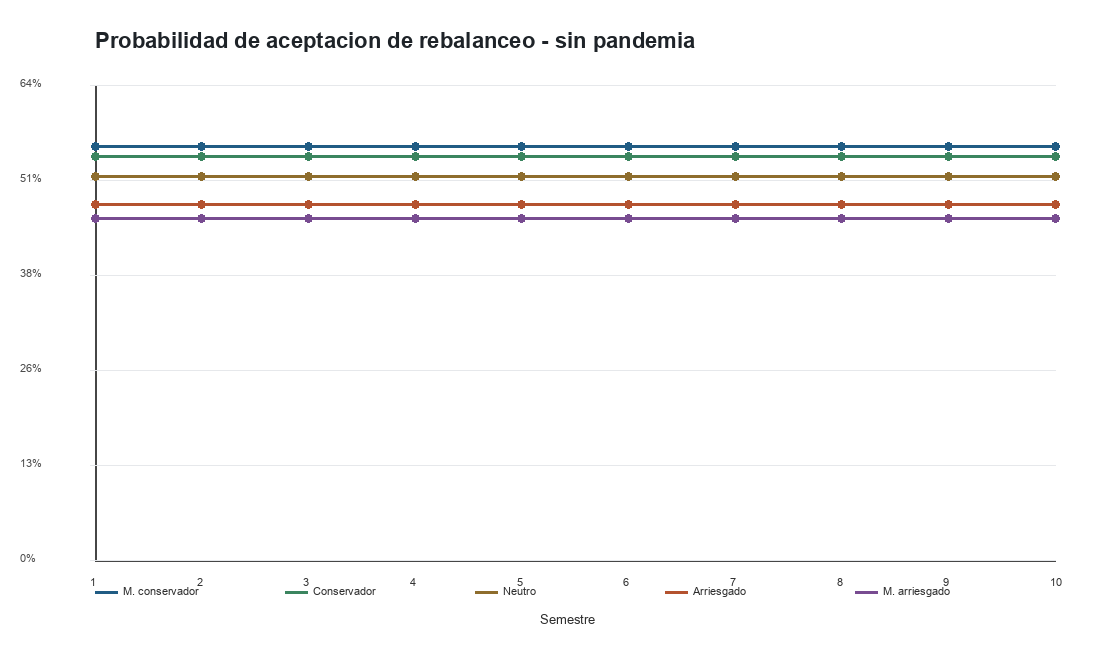
\includegraphics[width=0.86\textwidth]{figuras/serie_aceptacion_sin_pandemia.png}
\caption{Probabilidad semestral de aceptación de rebalanceo sin pandemia para Desempleo macro con abandono V1.}
\label{fig:desempleo_macro_v1:aceptacion_sin}
\end{figure}
\begin{figure}[H]
\centering
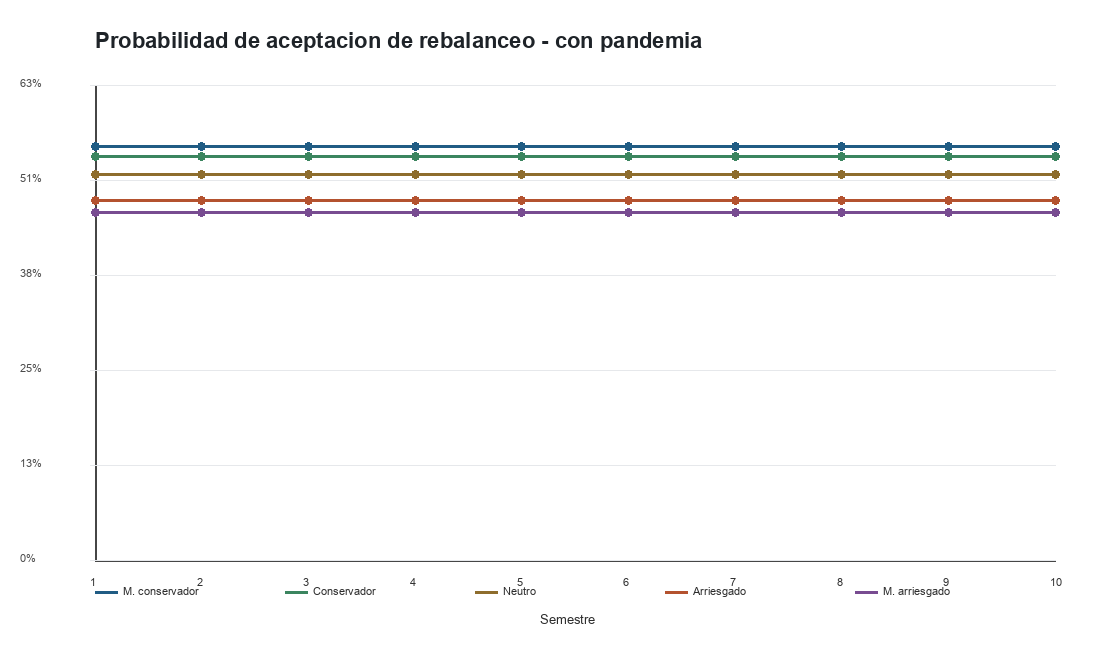
\includegraphics[width=0.86\textwidth]{figuras/serie_aceptacion_con_pandemia.png}
\caption{Probabilidad semestral de aceptación de rebalanceo con pandemia para Desempleo macro con abandono V1.}
\label{fig:desempleo_macro_v1:aceptacion_con}
\end{figure}
\begin{figure}[H]
\centering

\includegraphics[width=0.86\textwidth]{figuras/fig_probabilidades_sin_pandemia.png}
\caption{Probabilidades conductuales sin pandemia para Desempleo macro con abandono V1.}
\label{fig:desempleo_macro_v1:prob_sin}
\end{figure}
\begin{figure}[H]
\centering

\includegraphics[width=0.86\textwidth]{figuras/fig_probabilidades_con_pandemia.png}
\caption{Probabilidades conductuales con pandemia para Desempleo macro con abandono V1.}
\label{fig:desempleo_macro_v1:prob_con}
\end{figure}
\section{Discusión de Robustez}
La robustez se interpreta como la capacidad de sostener desempeno fuera de muestra, estabilidad de composicion y retencion de clientes bajo escenarios con y sin pandemia. La Version 1 elimina el abandono artificial cuando no hay exceso de perdida, pero mantiene una respuesta intensa cuando la perdida cruza la tolerancia.
\section{Conclusiones}
\begin{table}[H]
\centering
\resizebox{\textwidth}{!}{%
\begin{tabular}{lrrrrrrr}
\toprule
Perfil & Riqueza & Utilidad & P abandono sem. & Retiro 260w & Retencion & Clientes finales & Lectura \\
\midrule
Muy conservador & 1.374 & 114 & 15.2\% & 34.9\% & 37.3\% & 417 & Critica \\
Conservador & 1.774 & 242 & 1.7\% & 8.0\% & 85.4\% & 929 & Estable \\
Neutro & 1.827 & 259 & 0.0\% & 0.2\% & 99.6\% & 1029 & Estable \\
Arriesgado & 1.792 & 244 & 0.0\% & 0.0\% & 100.0\% & 955 & Estable \\
Muy arriesgado & 1.909 & 252 & 0.0\% & 0.1\% & 99.7\% & 925 & Estable \\
\bottomrule
\end{tabular}
}
\caption{Conclusion segmentada para Desempleo macro con abandono V1.}
\label{tab:desempleo_macro_v1:conclusiones}
\end{table}

La recomendacion final de esta view debe considerar simultaneamente mejora financiera, estabilidad dinamica y retencion. Cuando el modelo aumenta Sharpe pero exige alto turnover o concentra retornos en pocos sectores, su uso debe presentarse como tactico y condicionado al perfil de riesgo.
\end{document}